\chapter{\protect\hyperlink{:}{S Matrix and Scattering Theory}}
\addtocontents{toc}{\protect\hypertarget{:}{}}

\section{\protect\hyperlink{:}{S-matrix}}
\addtocontents{toc}{\protect\hypertarget{:}{}}



\subsection{\protect\hyperlink{:}{相互作用表象(interaction representation)}}
\addtocontents{toc}{\protect\hypertarget{:}{}}

在讲解 S 矩阵之前，我们需要先介绍一下相互作用表象的概念。我们知道在量子力学当中，我们有两种表象：海森堡表象和薛定谔表象，这两种表象分别对应着算符和态矢量的演化，但是海森堡表象当中算符是时间相关的而太矢量是时间无关的；薛定谔表象则相反，算符是时间无关的而态矢量是时间相关的，除了这两种表象外，为了描述相互作用，我们需要一种算符以及态矢量都随时间演化的表象，这就是相互作用表象。

在我们的理论当中，会有很多的接近于现实世界的一些模型，比如我们的谐振子还有自由粒子等等，但是它们终归不是真的符合现实世界的，因此，我们一般将现实的哈密顿量 $\hat{H}$ 给分成两部分，一部分是自由状态的哈密顿量 $ \hat{H}_0 $ ，而对于那些难以描述的所谓的复杂的过程，我们将其处理为相互作用项 $ \hat{H}^\prime $ ，同时对于自由项，其一定是随着时间演化的且易于求解的，因此我们认为在相互作用绘景下的算符将通过自由项 $ \hat{H}_0 $ 来演化的，即
\begin{equation}
    \hat{O}_I(t) = e^{i\hat{H}_0 t}\hat{O}e^{-i\hat{H}_0 t}
\end{equation} 

很显然，由于我们考虑的是自由项的哈密顿量的演化，所以他一定是遵循海森堡的算符的运动方程
\begin{equation}
    i \frac{d\hat{O}_I}{dt} = \left[\hat{O}_I(t) ,\hat{H}_0\right]
\end{equation}

但是这并没有包含有 $ \hat{H}^\prime $ ，因为一旦我们将其一并考虑进去，我们的态矢量也将一并随时间演化，这是海森堡绘景当中所不曾设计的，因此我们还需要将其与薛定谔绘景当中态矢量随时间演化相结合，可以得到
\begin{equation}
    \bra{\phi(t)}\hat{O}\ket{\psi(t)} = \bra{\phi_I(t)}\hat{O}_I\ket{\psi_I(t)}
\end{equation}

根据薛定谔绘景，我们可以得到
\begin{equation}
    \ket{\psi_I(t)} = e^{i\hat{H}_0 t}\ket{\psi(t)}
\end{equation}

接下来计算一下其关于时间的演化关系
\begin{eqnarray*}
    i\frac{d}{dt} \ket{\psi_I(t)} &=& e^{i\hat{H}_0 t}\left(-\hat{H}_0 + i\frac{d}{dt}\right)\ket{\psi(t)} \\
    &=& e^{i\hat{H}_0 t}\left(-\hat{H}_0 + \hat{H}\right)\ket{\psi(t)} \\
    &=& e^{i\hat{H}_0 t}\hat{H}^\prime\ket{\psi(t)} \\
    &=& e^{i\hat{H}_0 t}\hat{H}^\prime e^{-i\hat{H}_0 t}\ket{\psi_I(t)} \\
    &=& \hat{H}^\prime_I(t)\ket{\psi_I(t)}
\end{eqnarray*}

其中， $ \displaystyle \hat{H}_I(t) = e^{i\hat{H}_0 t}\hat{H}^\prime e^{-i\hat{H}_0 t} $ 

根据此，我们便可以定义出相互作用绘景：
\begin{enumerate}
    \item 算符和态矢量均随时间演化
    \item 算符的演化由非相互作用部分的哈密顿量所导致
    \item 态矢量的演化由相互作用部分的哈密顿量所导致
\end{enumerate}

\subsection{\protect\hyperlink{:}{The formular of S-matrix}}
\addtocontents{toc}{\protect\hypertarget{:}{}}

s-matirx 的想法由 John Wheeler 所提出，这个东西更像是一个时间演化算符，但不同的是他其中蕴含着散射的过程。

接下来我们给定两个粒子使其发生对心碰撞，接着这两个粒子在碰撞的那一瞬间发生了一系列的复杂反应并最终又以两个粒子散射出去，正如我们之前在相互作用绘景那一章所介绍的，我们一般将这样一个散射过程体系的哈密顿量拆分为两部分，一部分是无相互作用下的哈密顿量量外一部分是相互作用项的哈密顿量。需要注意的是，接下来我们是工作在 Heisenberg representation 的，所以记住我们的态矢量是不随时间演化的，那么对于简单世界（无相互作用）下的两个粒子其动量表象下的态矢量可以记作为 $ \ket{\psi} = \ket{p_2p_1}_{simpleworld} $ ，接着给出另外一个描述两个粒子在动量表象下的态矢量 $ \ket{\phi} = \ket{q_2q_1}_{simpleworld} $ ，与此同时，在现实世界当中给出一个存在的一个散射过程，当两个入射粒子一开始相距非常远的时候(可以认为是 $ t\to -\infty $ 的时候)我们给出一个态矢量 $ \ket{p_1p_2}_{realworld}^{in} $ ，当他们发生完散射之后，可能形成了两个（也有可能是多个或是一个，但这里我们假设是两个）粒子（可能并未发生改变，也有可能是全新的两个粒子），当他们相距非常远的时候(大概是 $ t \to \infty $ 的时候) 给出这个状态下的态矢量 $ \ket{q_1q_2}_{realworld}^{out} $ ，于是，我们可以通过让这两个态矢量作内积来得到这个散射过程的散射振幅 $ \mathcal{A} $  
\begin{equation}
    \mathcal{A} = ^{out}_{realworld}\braket{q_1q_2}{p_1p_2}_{realworld}^{in}
\end{equation}

但是这显然是很难计算出来的，为此我们需要寻找到在之前所定义的简单世界中的振幅与现实世界中的散射振幅之间的关系，为此，我们定义了 S-matrix
\begin{equation}
    \mathcal{A} = ^{out}_{realworld}\braket{q_1q_2}{p_1p_2}_{realworld}^{in} = _{simpleworld}\bra{q_1q_2}\hat{S}\ket{q_2q_1}_{simpleworld}
\end{equation}

因此，这个 $ \hat{S} $ 当中蕴含着我们想要从某个特定的初态到某一个特定的末态的散射振幅的信息，除此以外，为了能够计算出我们想要的散射振幅，我们还需要两样东西
\begin{enumerate}
    \item 找到一个合适的简单世界的哈密顿量 $ \hat{H}_0 $ 并以此来描述我们的类似与入态和出态的态矢量
    \item 计算出 $ \hat{S} $ 的表达形式的方法，这样我们才可以利用 $ _{simpleworld}\bra{q_1q_2}\hat{S}\ket{q_2q_1}_{simpleworld} $ 来计算出我们想要的散射振幅
\end{enumerate}


根据上面的讲解，我们知道所谓的入态和出态都是在时间处于无穷的时候，这也就是说在一开始，体系哈密顿量的相互作用项是可以忽略的，这种假设使得我们可以将 realworld 的态矢量写成 simpleworld 的态矢量，即
\begin{equation}
    \ket{\phi}_{simpleworld} = \ket{\phi_I(\pm \infty)}
\end{equation}

这意味着他们是 $ \hat{H}_0 $ 的本征矢量，因此，我们完全可以使用 $ \hat{H}_0 $ 的真空态以及产生湮灭算符来构建出我们的入态和出态.

随着时间的演化，慢慢的 $ \hat{H}_I $ 慢慢的将变得不可忽略，这也使得本征态的演化变得复杂起来，但到最后我们的 $ \hat{H}_I $ 将重新变得可以忽略，我们一般可以用一个系数来表示相互作用项占完整的哈密顿量的比例
\begin{figure}[ht]
\centering
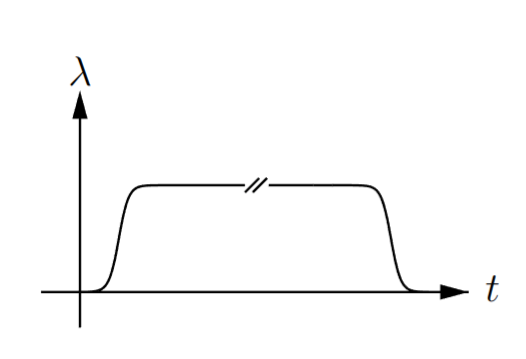
\includegraphics[width=0.4\textwidth]{figure/相互作用系数随时间的变化.png}
\caption{相互作用系数随时间的变化}
\label{fig1}
\end{figure}

如此一番定义，其实 $ \hat{S} $ 的形式已经昭然若揭，除此之外，我们还知道，当在初始时刻 $ t=0 $ 时，对于我们之前所提到的三个绘景，其测量应该是一样的，因此我们写出如下的式子，
\begin{eqnarray}
    _{simpleworld}\bra{\phi}\hat{S}\ket{\psi}_{simpleworld} &=& \braket{\phi_I(0)}{\psi_I(0)} \nonumber \\
    &=& \bra{\phi_I(\infty)}\hat{U}_I(\infty,0)\hat{U}_I(0,-\infty)\ket{\psi_I(-\infty)} \nonumber \\
    &=& \bra{\phi_I(\infty)}\hat{U}_I(\infty,-\infty)\ket{\psi_I(-\infty)}  \\
    &=& _{simpleworld}\bra{\phi}\hat{U}_I(\infty,-\infty)\ket{\psi}_{simpleworld}
\end{eqnarray}

据此，我们断言 $ \hat{S} $ 是相互作用绘景下的时间演化算符 $ \hat{U}_I(t,-t) $ 当 $ t \to \infty $ 的时候的极限。

所以，为了得到我们的 $ \hat{S} $ 的具体形式，我们还需要求解出相互作用绘景下的时间演化算符，在上上节当中我们有提到其方程
\begin{equation}
    i\frac{d}{dt}\hat{U}_I(t,t_0) = \hat{H}^\prime_I(t)\hat{U}_I(t,t_0)
\end{equation}

对于这个方程，我们可以通过不断的迭代求解出一个级数解
\begin{equation}
    \hat{U}_I(t,t_0) = 1 + \left(-i\right)\int_{t_0}^{t} dt_1\hat{H}_I(t_1) + \left(-i\right)^2 \int_{t_0}^{t}dt_1\int_{t_0}^{t_1}dt_2\hat{H}_I(t_1)\hat{H}_I(t_2) + \cdots
\end{equation}

通过观察这个展开式，我们可以发现其积分顺序是完全遵守时间从早到晚的顺序，这意味着我们可以使用 $ \hat{T} $ 来化简这个表达式
\begin{equation*}
    \left(-i\right)^2 \int_{t_0}^{t}dt_1\int_{t_0}^{t_1}dt_2\hat{H}_I(t_1)\hat{H}_I(t_2) = \frac{\left(-i\right)^2}{2} \int_{t_0}^{t}dt_1\int_{t_0}^{t}dt_2\hat{T}\left[\hat{H}_I(t_1)\hat{H}_I(t_2)\right]
\end{equation*}

\begin{figure}[ht]
    \centering
    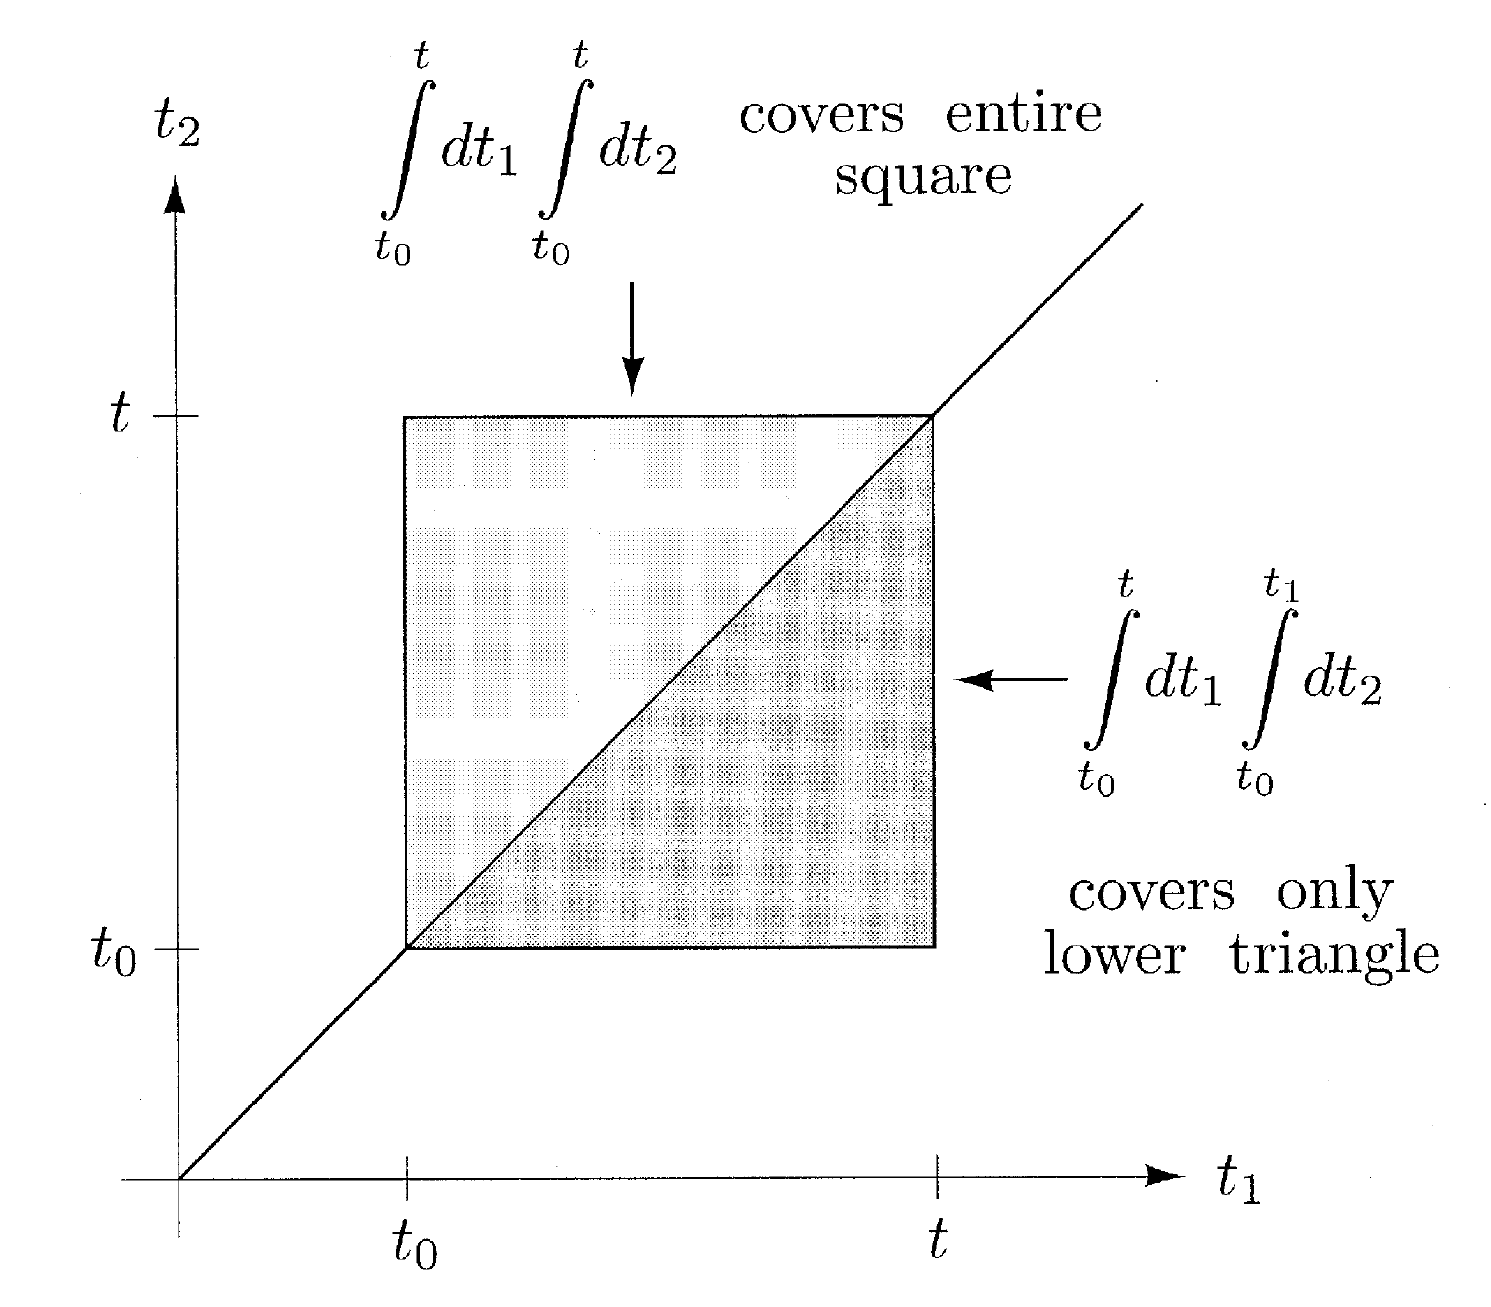
\includegraphics[width=0.6\textwidth]{figure/时间排序示意图.png}
    \label{fig2}
    \end{figure}

同理，剩余的部分我也可以用这样的方式来化简，最后我们得到
\begin{eqnarray*}
    &&\int_{t_0}^{t_1}dt_1\int_{t_0}^{t_2}dt_2\int_{t_0}^{t_3}dt_3 \cdots \int_{t_0}^{t_{n-1}} dt_n \hat{H}_I(t_1)\hat{H}_I(t_2)\cdots\hat{H}_I(t_n) \\
    &=&\frac{1}{A_n^n}\int_{t_0}^{t}dt_1\int_{t_0}^{t}dt_2\cdots\int_{t_0}^{t}dt_n \hat{T}\left[\hat{H}_I(t_1)\hat{H}_I(t_2)\cdots\hat{H}_I(t_n)\right]
\end{eqnarray*}

求和可以得到相互作用绘景下的时间演化算符
\begin{equation}
    \hat{U}_I(t,t_0) = T\left\{\exp\left[-i\int_{t_0}^{t}dt^\prime \hat{H}_I(t^\prime)\right]\right\}
\end{equation}



终于，可以将 $ \hat{S} $ 求解出来了
\begin{equation*}
    \hat{S} = T\left\{\exp\left[-i\int_{-\infty}^{+\infty}dt^\prime \hat{H}_I(t^\prime)\right]\right\}
\end{equation*}

转化为哈密顿量密度，得到
\begin{equation}
    \hat{S} = T\left\{\exp\left[-i\int_{-\infty}^{+\infty}d^4x \hat{H}_I(x)\right]\right\}
\end{equation}

\begin{equation}
    \wick{
        \c1 \phi_1^+ (x)  \c1 \phi_1^- (y)
    }
\end{equation}




\section{\protect\hyperlink{:}{Wick 定理与费曼图}}
\addtocontents{toc}{\protect\hypertarget{:}{}}

\subsection{\protect\hyperlink{:}{Why Wick's Theorm}}
\addtocontents{toc}{\protect\hypertarget{:}{}}

从之前的讨论当中，我们知道想要去计算出散射振幅，求解
\begin{equation}
    \bra{0}\hat{S}\ket{0} = \left\langle 0 \left|T\left\{\exp\left[-i\int_{-\infty}^{+\infty}d^4x \hat{H}_I(x)\right]\right\}\right|0\right\rangle
\end{equation}

我们可以通过围绕展开的方式求解 $ \left\langle 0 \left|T\left\{\exp\left[-i\int_{-\infty}^{+\infty}d^4x \hat{H}_I(x)\right]\right\}\right|0\right\rangle $ 

\begin{equation}
    \hat{S} = T\left[1 - i\int d^4 z \hat{\mathcal{H}}_I(z) + \frac{(-i)^2}{2!} d^4y d^4w \hat{\mathcal{H}}_I(y) \hat{\mathcal{H}}_I(w) + \cdots\right]
\end{equation}

这意味着我们需要去求解形如这样的真空期望值
\begin{equation}
    \bra{0}T[\hat{A}\hat{B}\cdots\hat{Z}]\ket{0}
\end{equation}

可是，我们需要根据这一系列算符的时间顺序来求解，很显然，这是费时费力并且容易出错的，因此我们必须寻求一个简单的方法来求解真空期望值，这就不得不回想起之前所得到的一种排序算符 $N$，
\begin{equation}
    \bra{0}N[\hat{A}\hat{B}\cdots\hat{Z}]\ket{0}
\end{equation}

这是非常容易计算的，我们只需要将产生算符放在湮灭算符的左边就行，例如对于一个场算符 $\hat{\phi}$ ,其是由产生算符和湮灭算符构成的 $\hat{\phi} = \hat{\phi}^+ \hat{\phi}^-$ ，因此，我们有 $\hat{\phi}^-\ket{0} = 0 , \bra{0}\hat{\phi}^+ = 0$ ，根据这个，我们先考虑一个最简单的情况，找一找 $\bra{0}T[\hat{A}\hat{B}]\ket{0}$ 和 $\bra{0}N[\hat{A}\hat{B}]\ket{0}$ 之间的关系，

首先计算一下 $\hat{A}\hat{B}$
\begin{equation}
    \hat{A}\hat{B} = \left(\hat{A}^+ + \hat{A}^-\right)\left(\hat{B}^+ + \hat{B}^-\right) = \hat{A}^+\hat{B}^+ + \hat{A}^+\hat{B}^- + \hat{A}^-\hat{B}^+ + \hat{A}^-\hat{B}^-
\end{equation}

通过使用 normal ordering ，可以得到 
\begin{equation}
    N[\hat{A}\hat{B}] = \hat{A}^+\hat{B}^+ + \hat{A}^-\hat{B}^- + \hat{A}^+\hat{B}^- + \hat{B}^+\hat{A}^-
\end{equation}

给出 $\hat{A}\hat{B}$ 与 $N[\hat{A}\hat{B}]$ 之间的不同
\begin{equation}
    \hat{A}\hat{B} - N[\hat{A}\hat{B}] = \hat{A}^-\hat{B}^+ + \hat{B}^+\hat{A}^- = [\hat{A}^-,\hat{B}^+]
\end{equation}

基于此，先给出 $T[\hat{A}(x)\hat{B}(y)]$ 的形式
\begin{equation}
    T[\hat{A}(x)\hat{B}(y)] = 
    \begin{cases}
        \hat{A}(x)\hat{B}(y) &\quad x^0 < y^0 \\
        \hat{B}(y)\hat{A}(x) &\quad x^0 > y^0 
    \end{cases}
\end{equation}

可以发现，貌似有个规律
\begin{equation}
    T[\hat{A}(x)\hat{B}(y)] - N[\hat{A}(x)\hat{B}(y)] = 
    \begin{cases}
        [\hat{A}^-(x)\hat{B}^+(y)] &\quad x^0 < y^0 \\
        [\hat{B}^-(y)\hat{A}^+(x)] &\quad x^0 > y^0
    \end{cases}
\end{equation}

之前有提到过，$\hat{\phi}^-\ket{0} = 0 , \bra{0}\hat{\phi}^+ = 0$，因此，我们的 normal ordering 的真空期望值为 $0$，于是，我们可以得到关系
\begin{equation}
    \bra{0}T[\hat{A}(x)\hat{B}(y)]\ket{0} = 
    \begin{cases}
        \bra{0}[\hat{A}^-(x)\hat{B}^+(y)]\ket{0} &\quad x^0 < y^0 \\
        \bra{0}[\hat{B}^-(y)\hat{A}^+(x)]\ket{0} &\quad x^0 > y^0
    \end{cases}
\end{equation}

如果我们在这个时候取 $\hat{A} = \hat{B} = \phi$ ，那么该真空期望值将会刚刚好是费曼传播子，当然，我们也为此定义出一个新的运算 $\mathbf{contraction}$ (说真的，不知道为什么这个 $simpler-wick$ 宏包没办法敲进去 $\hat{A}$ 和 $\hat{B}$)。

\begin{equation}
    \wick{
        \c1 A   \c1 B
    } = T[\hat{A}\hat{B}] - N[\hat{A}\hat{B}]
\end{equation}

从上面的式子当中，我们可以知道，这个 contraction 是一个对易子，并且该对易子当中均为产生湮灭算符，于是我们可以将其使用自由标量场理论 $\hat{\phi},\partial_\mu \hat{\phi},\hat{\phi}^2$ 将其表示出来,并通过最为基本的产生湮灭算符 $\hat{a}_p,\hat{a}_{p}^\dagger$，即 
\begin{eqnarray*}
    \hat{A}^{-} &=& \sum_i \alpha_i \hat{a}_i \\
    \hat{B}^{+} &=& \sum_i \beta_i \hat{a}_i^\dagger
\end{eqnarray*}

可以简单计算到，对于 $[\hat{A}^-,\hat{B}^+] = \hat{A}^-\hat{B}^+ - \hat{B}^+\hat{A}^-$
\begin{equation}
    \hat{A}^-\hat{B}^+ - \hat{B}^+\hat{A}^- = \alpha_i \beta_j \left(\hat{a}_i \hat{a}_j^\dagger - \hat{a}_j^\dagger\hat{a}_i\right) = \alpha_i \beta_j [\hat{a}_j^\dagger,\hat{a}_i] = \alpha_i \beta_j \delta_{ij} = \alpha_i \beta_i
\end{equation}

同理 $[\hat{B}^-,\hat{A}^+]$ 也是如此，这也就是说我们的 contraction 是一个 c-number ，故
\begin{equation}
    \wick{
        \c1 A   \c1 B
    } = 
    \wick{
        \c1 A   \c1 B
    }\braket{0}{0} =
    \bra{0}
    \wick{
        \c1 A   \c1 B
    }\ket{0} = 
    \bra{0}T[\hat{A}\hat{B}]\ket{0}
\end{equation}

除此以外，由于 $\wick{\c1 A \c1 B}$ 经过证明是一个 c-number ，所以我们的 $N,T$ 对他来说并不会产生什么直接的作用，也就是说
\begin{equation}
    T[\hat{A}\hat{B}] = N[\hat{A}\hat{B}] + \wick{\c1 A \c1 B} = N[\hat{A}\hat{B} + \wick{\c1 A \c1 B}]
\end{equation}

扩展到多个算符，那么我们将会有
\begin{theorem}{Wick's Theorm}
    \begin{equation}
        T[\hat{A}\hat{B}\hat{C}\cdots\hat{Z}] = N\left[\hat{A}\hat{B}\hat{C}\cdots\hat{Z} + \ all\ possible\ constraction\ of\ \hat{A}\hat{B}\hat{C}\cdots\hat{Z}\right]
    \end{equation}
\end{theorem}


OK,有了这样一个利器，我们将可以更加容易的完成对于 $T[\cdots]$ 的真空期望值的计算，接下来我们给出一个例子来见识到我们的 Wick's Theorm 的强大力量。
\begin{example}
    求解一下 $T[\hat{A}\hat{B}\hat{C}\hat{D}]$ 的真空期望值。
    \begin{solution}
        \begin{eqnarray*}
            T[\hat{A}\hat{B}\hat{C}\hat{D}] &=& N[\hat{A}\hat{B}\hat{C}\hat{D}] + N[\wick{\c1 A \c1 B C D}] + N[\wick{\c1 A B \c1 C D}] + N[\wick{\c1 A B C \c1 D}] + N[\hat{A}\wick{\c1 B \c1 C}\hat{D}] + N[\wick{A \c1 B C \c1 D}] + N[\hat{A}\hat{B}\wick{\c1 C \c1 D}] \\
            && + N[\wick{\c1 A \c1 B \c2 C \c2 D}] + N[\wick{\c1 A \c2 B \c1 C \c2 D}] + N[\wick{\c1 A \c2 B \c2 C \c1 D}]
        \end{eqnarray*}

        我们也不能忘记，在之前，就已经证明出 contraction 是一个 c-number ，因此我们是完全可以将其从 normal ordering 当中提取出来的，同时，考虑到 $\bra{0}N[\cdots]\ket{0} = 0$ ,我们可以知道，只有当 normal ordering 当中全部都变成了constration 的时候，其才会对真空期望值产生一定的贡献(对于我们目前计算的，就是指第二行的三个量)，于是我们可以得到
        \begin{eqnarray*}
            \left\langle 0 \left|T[\hat{A}\hat{B}\hat{C}\hat{D}]\right|0 \right\rangle &=& \left\langle 0 \left|T[\hat{A}\hat{B}]\right|0 \right\rangle\left\langle 0 \left|T[\hat{C}\hat{D}]\right|0 \right\rangle + \left\langle 0 \left|T[\hat{A}\hat{C}]\right|0 \right\rangle\left\langle 0 \left|T[\hat{B}\hat{D}]\right|0 \right\rangle + \left\langle 0 \left|T[\hat{A}\hat{D}]\right|0 \right\rangle\left\langle 0 \left|T[\hat{B}\hat{C}]\right|0 \right\rangle
        \end{eqnarray*} 
    \end{solution}
\end{example}

基于如上例子所计算出来的结果，我们将其运用到场算符之上
\begin{eqnarray*}
    \left\langle 0 \left|T[\hat{\phi}(x_1)\hat{\phi}(x_2)\hat{\phi}(x_3)\hat{\phi}(x_4)]\right|0 \right\rangle &=& \left\langle 0 \left|\hat{\phi}(x_1)\hat{\phi}(x_2)\hat{\phi}(x_3)\hat{\phi}(x_4)\right|0 \right\rangle \\
    &=& \left\langle 0 \left|T[\hat{\phi}(x_1)\hat{\phi}(x_2)]\right|0 \right\rangle\left\langle 0 \left|T[\hat{\phi}(x_3)\hat{\phi}(x_4)]\right|0 \right\rangle + \left\langle 0 \left|T[\hat{\phi}(x_1)\hat{\phi}(x_3)]\right|0 \right\rangle\left\langle 0 \left|T[\hat{\phi}(x_2)\hat{\phi}(x_4)]\right|0 \right\rangle \\
    &+& \left\langle 0 \left|T[\hat{\phi}(x_1)\hat{\phi}(x_4)]\right|0 \right\rangle\left\langle 0 \left|T[\hat{\phi}(x_2)\hat{\phi}(x_3)]\right|0 \right\rangle
\end{eqnarray*}

根据我们之前所提到的标量场的费曼传播子形式是一致的，于是我们有
\begin{equation*}
    \left\langle 0 \left|\hat{\phi}(x_1)\hat{\phi}(x_2)\hat{\phi}(x_3)\hat{\phi}(x_4)\right|0 \right\rangle = \Delta(x_1 - x_2)\Delta(x_3 - x_4) + \Delta(x_1 - x_3)\Delta(x_2 - x_4) + \Delta(x_1 - x_4)\Delta(x_2 - x_3)
\end{equation*}

很显然，wick's theorem 给我们计算真空期望值带来了很大的便利以及非常直观的物理图像，接下来我们需要做的，就是去计算我们的 $\hat{S}$ 矩阵。


\subsection{\protect\hyperlink{:}{Expanding the S-matrix by Wick's Theorm}}
\addtocontents{toc}{\protect\hypertarget{:}{}}

首先给定几个符号规则

\begin{table}[hbpt]
\begin{minipage}{0.5\textwidth}
    \centering
    \begin{tikzpicture}
        \begin{feynman}
          % 顶点
          \vertex (a) at (0,0) {$\bigcirc $};
          \vertex [right=2cm of a] (b);
          
          % 粒子线
          \diagram* {
            (a) -- [solid,edge label=$\phi(z)$] (b)
          };
        \end{feynman}
    \end{tikzpicture}
\end{minipage}
\hfill
\begin{minipage}{0.5\textwidth}
    这是最简单的相互作用哈密顿量 $\hat{H}_I(z)$,它包含一个标量场 $\phi(z)$ 和一个源场 $J(z)$,
    \begin{equation*}
        \hat{H}_I(z) = J(z)\phi(z)
    \end{equation*}
\end{minipage}
\end{table}

\begin{table}[hbpt]
    \begin{minipage}{0.5\textwidth}
        \centering
        \begin{tikzpicture}
            \begin{feynman}
                \vertex (a) {$\bullet$};
                \vertex [above right=2cm of a] (b){$\phi(z)$};
                \vertex [below right=2cm of a] (c){$\phi(z)$};
                \vertex [above left=2cm of a] (d){$\phi(z)$};
                \vertex [below left=2cm of a] (e){$\phi(z)$};

                \diagram* {
                    (a) -- [solid] (b),
                    (a) -- [solid] (c),
                    (a) -- [solid] (d),
                    (a) -- [solid] (e)
                };
            \end{feynman}
        \end{tikzpicture}
    \end{minipage}
    \hfill
    \begin{minipage}{0.5\textwidth}
        这是最简单的自相互作用哈密顿量 $\hat{H}_I(z)$,我们一般将其称之为 $\phi^4$ 理论，其相互作用部分的哈密顿量为
        \begin{equation*}
            \hat{H}_I(z) = \frac{\lambda}{4!}\phi^4(z)
        \end{equation*}
    \end{minipage}
\end{table}

\begin{table}[hbpt]
    \begin{minipage}{0.5\textwidth}
        \centering
        \begin{tikzpicture}
            \begin{feynman}
                \vertex (a) ;
                \vertex [right=2cm of a] (b){$\phi(z)$};
                \vertex [above left=2cm of a] (c){$\psi^\dagger(z)$};
                \vertex [below left=2cm of a] (d){$\psi(z)$};
                \diagram* {
                    (a) -- [solid] (b),
                    (c) -- [anti fermion] (a),
                    (d) -- [fermion] (a)
                };
            \end{feynman}
        \end{tikzpicture}
    \end{minipage}
    \hfill
    \begin{minipage}{0.5\textwidth}
        这种相互作用是由 YuKawa 所提出的，其相互作用部分的哈密顿量 $\hat{H}_I(z)$为
        \begin{equation*}
            \hat{H}_I(z) = g \psi^\dagger(z)\psi(z)\phi(z)
        \end{equation*}
    \end{minipage}
\end{table}

\begin{table}[hbpt]
    \begin{minipage}{0.5\textwidth}
        \centering
        \begin{tikzpicture}
            \begin{feynman}
                \vertex (a) ;
                \vertex [right=2cm of a] (b);
                \vertex [above left=2cm of a] (c){$\psi^\dagger(x)$};
                \vertex [below left=2cm of a] (d){$\psi(x)$};
                \vertex [above right=2cm of b] (e){$\psi^\dagger(y)$};
                \vertex [below right=2cm of b] (f){$\psi(y)$};
                \diagram* {
                    (a) -- [boson,edge label=$V(x - y)$] (b),
                    (c) -- [anti fermion] (a),
                    (d) -- [fermion] (a),
                    (e) -- [anti fermion] (b),
                    (f) -- [fermion] (b)
                };
            \end{feynman}
        \end{tikzpicture}
    \end{minipage}
    \hfill
    \begin{minipage}{0.5\textwidth}
        最后一个例子是一种非常有用的非相对论的相互作用，其可以用来描述库伦相互作用，其相互作用部分的哈密顿量 $\hat{H}_I(z)$为
        \begin{equation*}
            \hat{H}_I(z) = \frac{1}{2}\psi^\dagger(x)\psi^\dagger(y)V(x - y)\delta(x^0 - y^0)\psi(y)\psi(x)
        \end{equation*}
    \end{minipage}
\end{table}

在介绍完一些相互作用以及图形上的表示之后，我们将会以 $\phi^4$ 相互作用作为例子来展开 \\
$T[\hat{\phi}(x_1)\hat{\phi}(x_2)\hat{\phi}(x_3)\hat{\phi}(x_4)]$ 的真空期望值，首先，给出该相互作用的拉格朗日量
\begin{equation}
    \mathcal{L} = \frac{1}{2}\left[\partial_\mu \phi(x)\right]^2 - \frac{1}{2}m^2\phi^2(x) - \frac{\lambda}{4!}\phi^4(x)
\end{equation}

该拉格朗日量其前面一部分为自由 Klein-Gordon 场的拉格朗日量，我们可以将这部分通过正则量子化的方法得到系统的哈密顿量
\begin{equation}
    \hat{\mathcal{H}}_0 = \frac{1}{2}\left[\left(\frac{\partial \hat{\phi}}{\partial t}\right)^2 + \left(\nabla\hat{\phi}\right)^2 + m^2\hat{\phi}^2\right] 
\end{equation}

而相互作用部分的哈密顿量则为
\begin{equation}
    \hat{\mathcal{H}}_I = \frac{\lambda}{4!}\phi^4(x)
\end{equation}

接下来，给出一个具体的过程来展开一下这个过程的 $\hat{S}$ 矩阵
\begin{example}
    考虑一个过程，其入态为一个处于 $p$ 的动量本征态的粒子，而其出态为一个处于 $q$ 的动量本征态的粒子，接下来计算一下这个过程的振幅
    \begin{solution}
        \begin{enumerate}
            \item[Step 1] 计算一下振幅 $\mathcal{A}$
            \begin{equation}
                \mathcal{A} = ^{out}\braket{q}{p}^{in} = \bra{q}\hat{S}\ket{p} = (2\pi)^3 \left(2E_{\vec{q}}\right)^{\frac{1}{2}} \left(2E_{\vec{p}}\right)^{\frac{1}{2}}\bra{0}\hat{a}_{\vec{q}}\hat{S}\hat{a}_{\vec{p}}^\dagger\ket{0}
            \end{equation}

            其中，我们的$\displaystyle \ket{p} = (2\pi)^\frac{3}{2} \left(2E_{\vec{p}}\right)^{\frac{1}{2}}\hat{a}_{\vec{p}}^\dagger\ket{0}$
            \item[Step 2] 将 $\hat{S}$ 从 Dyson's 表示进行展开，从而得到
            \begin{equation}
                \hat{S} = T\left[1 - \frac{i\lambda}{4!}\int d^4z \hat{\phi}^4(z) + \frac{\left(-i\right)^2}{2!}\left(\frac{\lambda}{4!}\right)^2 \int d^4 x d^4 y \hat{\phi}^4(x)\hat{\phi}^4(y) + \cdots\right]
            \end{equation}
            \item[Step 3] 将我们展开之后的 $\hat{S}$ 代入到 $\mathcal{A}$ 当中
            \begin{eqnarray*}
                \mathcal{A} &=& \bra{q}\hat{S}\ket{p} \\
                &=& (2\pi)^3 \left(2E_{\vec{q}}\right)^{\frac{1}{2}} \left(2E_{\vec{p}}\right)^{\frac{1}{2}} T\left[\bra{0}\hat{a}_{\vec{q}}\hat{a}_{\vec{p}}^\dagger\ket{0} + \int d^4z \left(\frac{-i\lambda}{4!}\right)\bra{0}\hat{a}_{\vec{q}}\hat{\phi}^4(z)\hat{a}_{\vec{p}}^\dagger\ket{0}\right. \\
                && \left. + \int d^4x d^4y \frac{1}{2!}\left(\frac{-i\lambda}{4!}\right)^2\bra{0}\hat{a}_{\vec{q}}\hat{\phi}^4(x)\hat{\phi}^4(y)\hat{a}_{\vec{p}}^\dagger\ket{0} + \cdots\right]
            \end{eqnarray*}

            于是，我们可以很自然的将振幅按照 $\lambda$ 的幂次来划分写作每一阶振幅的总和，即
            \begin{equation}
                \mathcal{A} = \mathcal{A}^{(0)} + \mathcal{A}^{(1)} + \mathcal{A}^{(2)} + \mathcal{A}^{(3)} + \cdots
            \end{equation}
            \item[Step 4] 得到了展开后的振幅之后，我们可以看出，真空期望值我们完全可以使用上一节得到的 Wick's Theorm 来展开，接下来开始
            \begin{itemize}
                \item 计算领头阶（LO）的真空期望值，这很容易
                \begin{equation*}
                    \mathcal{A}^{(0)} \propto T\left[\bra{0}\hat{a}_{\vec{q}}\hat{a}_{\vec{p}}^\dagger\ket{0}\right] = \wick{\c1 a_{\vec{q}} \c1 a_{\vec{p}}} = \delta^{(3)}(\vec{q} - \vec{p})
                \end{equation*}
                \item 计算一下较为复杂的次领头阶（NLO）振幅当中的真空期望值，通过 wick constraction 我们可以得到
                \begin{eqnarray*}
                    \mathcal{A}^{(1)} &\propto& \int d^4z \left(\frac{-i\lambda}{4!}\right)\bra{0}T[\hat{a}_{\vec{q}}\hat{\phi}^4(z)\hat{a}_{\vec{p}}^\dagger]\ket{0} \\
                    &=& \int d^4z \left(\frac{-i\lambda}{4!}\right)\left[3 \bra{0} \hat{a}_{\vec{q}}\hat{a}_{\vec{p}}^\dagger\ket{0}\bra{0} \hat{\phi}(x)\hat{\phi}(x) \ket{0}\bra{0} \hat{\phi}(x)\hat{\phi}(x) \ket{0} \right. \\
                    &+& \left.12 \bra{0} \hat{a}_{\vec{q}}\hat{\phi}\ket{0}\bra{0} \hat{\phi}\hat{\phi}\ket{0}\bra{0} \hat{\phi}\hat{a}_{\vec{p}}^\dagger\ket{0} \right]
                \end{eqnarray*}

                这很复杂（至少对我来说），我们需要分别计算一下这里面出现的几个真空期望值,借用一下之前的结论（我们考虑的是一个自由标量场的 $\phi^4$ 理论），其场算符在 $\ket{p}$ 的动量本征态下的形式为
                \begin{equation}
                    \hat{\phi}(z) = \int \frac{d^3 \vec{p}}{\left(2\pi\right)^{\frac{3}{2}}} \frac{1}{\left(2 E_{\vec{p}}\right)^{\frac{1}{2}}}\left(\hat{a}_{\vec{p}}e^{-ip \cdot z} + \hat{a}_{\vec{p}}^\dagger e^{ip \cdot z}\right)
                \end{equation}

                根据该场算符的形式，我们可以计算得到
                \begin{eqnarray*}
                    \bra{0} \hat{\phi}(z)\hat{\phi}(z) \ket{0} &=& \Delta(z - z)\\
                    &=& \int \frac{d^4 k}{(2\pi)^4} \frac{e^{-ik(z - z)}}{k^2 - m^2 + i\epsilon}\\
                    \bra{0} \hat{a}_{\vec{q}}\hat{\phi}(z) \ket{0} &=& \int d^3 \vec{q}^\prime d^3 \vec{p}^\prime \braket{\vec{q}}{\vec{p}^\prime}e^{i p^\prime \cdot z} \\
                    &=& e^{iq\cdot z} \\
                    \bra{0} \hat{\phi}(z)\hat{a}_{\vec{p}}^\dagger \ket{0} &=& e^{-ip\cdot z}
                \end{eqnarray*}

                其中，$\bra{0} \hat{\phi}(z)\hat{\phi}(z) \ket{0} = \Delta(0)$ 对应的是所谓的 tadpole 图（蝌蚪图），它是一个与外动量无关的常数，可以通过正规化重整化来消除。而 $\bra{0} \hat{a}_{\vec{q}}\hat{\phi}(z) \ket{0}$ 和 $\bra{0} \hat{\phi}(z)\hat{a}_{\vec{p}}^\dagger \ket{0}$ 则分别对应着外线与顶点的连接。

                \item[Step 5] 将所有结果组合起来，我们得到 NLO 振幅
                \begin{eqnarray*}
                    \mathcal{A}^{(1)} &=& \int d^4z \left(\frac{-i\lambda}{4!}\right)\left[12 \cdot e^{iq\cdot z} \cdot \Delta(0) \cdot e^{-ip\cdot z}\right] \\
                    &=& -i\lambda \cdot \Delta(0) \int d^4z \, e^{i(q-p)\cdot z} \\
                    &=& -i\lambda \cdot \Delta(0) \cdot (2\pi)^4 \delta^{(4)}(q - p)
                \end{eqnarray*}

                这个结果告诉我们，NLO 的贡献正比于 $\lambda$ 以及 $\Delta(0)$，并且含有动量守恒的 $\delta$ 函数。$\Delta(0)$ 对应的是一个圈图（loop）贡献，这正是微扰论中需要处理的发散问题的来源之一。

                \item[Step 6] 接下来计算次次领头阶（NNLO，$\mathcal{O}(\lambda^2)$）的振幅，这将展示 Wick 定理处理更复杂收缩的能力
                \begin{eqnarray*}
                    \mathcal{A}^{(2)} &\propto& \int d^4x d^4y \frac{1}{2!}\left(\frac{-i\lambda}{4!}\right)^2 \bra{0}T[\hat{a}_{\vec{q}}\hat{\phi}^4(x)\hat{\phi}^4(y)\hat{a}_{\vec{p}}^\dagger]\ket{0}
                \end{eqnarray*}

                这里出现了 $8$ 个场算符和 $2$ 个湮灭/产生算符的 Wick 收缩。让我们系统地分析所有可能的收缩方式。

                首先，将场算符明确写出：
                \begin{eqnarray*}
                    \hat{\phi}^4(x)\hat{\phi}^4(y) &=& \phi(x_1)\phi(x_2)\phi(x_3)\phi(x_4)\phi(y_1)\phi(y_2)\phi(y_3)\phi(y_4)
                \end{eqnarray*}
                其中 $x_i$ 和 $y_j$ 都代表同一个时空点 $x$ 和 $y$，只是为了标记区分。

                我们需要将 $\hat{a}_{\vec{q}}$ 和 $\hat{a}_{\vec{p}}^\dagger$ 与场算符收缩，同时将剩余的场算符两两配对。根据收缩的拓扑结构，可以分为两大类：

                \textbf{(a) 连通图（Connected diagram）：}

                入态和出态粒子分别连接到不同的顶点（或同一顶点），且两个顶点通过传播子连接。

                \textbf{情况1}：$\hat{a}_{\vec{q}}$ 与 $\phi(x)$ 收缩，$\hat{a}_{\vec{p}}^\dagger$ 与 $\phi(y)$ 收缩
                \begin{itemize}
                    \item $\hat{a}_{\vec{q}}$ 选择 $\phi(x)$ 的方式有 $4$ 种
                    \item $\hat{a}_{\vec{p}}^\dagger$ 选择 $\phi(y)$ 的方式有 $4$ 种
                    \item 剩余的 $3$ 个 $\phi(x)$ 和 $3$ 个 $\phi(y)$ 需要两两配对
                    \item 其中必须有一个 $\phi(x)$ 与一个 $\phi(y)$ 收缩形成传播子 $\Delta_F(x-y)$
                    \item 剩余的 $2$ 个 $\phi(x)$ 自收缩形成 $\Delta(0)$，剩余的 $2$ 个 $\phi(y)$ 自收缩形成 $\Delta(0)$
                \end{itemize}

                计算对称性因子：
                \begin{itemize}
                    \item 选择哪个 $\phi(x)$ 与 $\phi(y)$ 收缩：$3 \times 3 = 9$ 种
                    \item 剩余 $\phi(x)$ 的配对方式：$1$ 种（只有 $2$ 个，只能自收缩）
                    \item 剩余 $\phi(y)$ 的配对方式：$1$ 种
                \end{itemize}

                因此，这种情况的贡献为：
                \begin{eqnarray*}
                    4 \times 4 \times 9 &=& 144
                \end{eqnarray*}

                \textbf{情况2}：$\hat{a}_{\vec{q}}$ 和 $\hat{a}_{\vec{p}}^\dagger$ 都与同一个顶点（比如 $\phi(x)$）收缩
                \begin{itemize}
                    \item $\hat{a}_{\vec{q}}$ 选择 $\phi(x)$ 的方式有 $4$ 种
                    \item $\hat{a}_{\vec{p}}^\dagger$ 选择剩余 $\phi(x)$ 的方式有 $3$ 种
                    \item 剩余的 $2$ 个 $\phi(x)$ 自收缩形成 $\Delta(0)$
                    \item $4$ 个 $\phi(y)$ 两两收缩，形成 $2$ 个 $\Delta(0)$ 或 $1$ 个 $\Delta_F(x-y)$ 的环
                \end{itemize}

                这种情况对应着入态和出态粒子从同一顶点进入，然后通过传播子连接到另一个顶点。

                综合所有连通图的贡献，我们得到：
                \begin{eqnarray*}
                    \wick{\c1 a_{\vec{q}} \c2 \phi \c3 \phi \c4 \phi \c5 \phi \c6 \phi \c7 \phi \c8 \phi \c9 \phi \c1 a_{\vec{p}}^\dagger} \Big|_{\text{connected}} &=& C_{\text{conn}} \cdot e^{iq\cdot x} \cdot \Delta_F(x-y) \cdot e^{-ip\cdot y} \cdot \left[\Delta(0)\right]^2
                \end{eqnarray*}

                其中 $C_{\text{conn}}$ 是所有连通图贡献的总系数。

                \textbf{(b) 非连通图（Disconnected diagram）：}

                入态和出态粒子直接传播，不与相互作用顶点相连：
                \begin{eqnarray*}
                    \wick{\c1 a_{\vec{q}} \c2 \phi \c3 \phi \c4 \phi \c5 \phi \c6 \phi \c7 \phi \c8 \phi \c9 \phi \c1 a_{\vec{p}}^\dagger} \Big|_{\text{disconnected}} &=& e^{iq\cdot x} e^{-ip\cdot y} \cdot \left[\Delta(0)\right]^4
                \end{eqnarray*}

                这对应着一个非连通图：入态粒子直接传播到出态，与相互作用完全无关，另外还有两个独立的真空涨落圈。

                \item[Step 7] 将 NNLO 的结果组合起来

                考虑到所有的对称性因子和 $\frac{1}{2!}\left(\frac{-i\lambda}{4!}\right)^2$ 的系数，我们得到
                \begin{eqnarray*}
                    \mathcal{A}^{(2)} &=& \frac{1}{2!}\left(\frac{-i\lambda}{4!}\right)^2 \int d^4x d^4y \Big[ C_{\text{conn}} \cdot e^{iq\cdot x} \Delta_F(x-y) e^{-ip\cdot y} \left(\Delta(0)\right)^2 \\
                    &+& C_{\text{disc}} \cdot e^{iq\cdot x} e^{-ip\cdot y} \left(\Delta(0)\right)^4 \Big]
                \end{eqnarray*}

                做傅里叶变换到动量空间，我们得到
                \begin{eqnarray*}
                    \mathcal{A}^{(2)} &=& \frac{(-i\lambda)^2}{2} \cdot C_{\text{conn}} \cdot \frac{i}{(q-p)^2 - m^2 + i\epsilon} \cdot \left[\Delta(0)\right]^2 \cdot (2\pi)^4\delta^{(4)}(q-p) \\
                    &+& \frac{(-i\lambda)^2}{2} \cdot C_{\text{disc}} \cdot \left[\Delta(0)\right]^4 \cdot (2\pi)^4\delta^{(4)}(q-p)
                \end{eqnarray*}
            \end{itemize}

            \item[Step 8] 物理意义分析

            从上面的计算我们可以看到几个重要的物理图像：

            \begin{enumerate}
                \item \textbf{连通与非连通}：非连通图（vacuum bubble）不参与散射过程，可以通过正规化消除。物理上可观测的散射振幅只来自连通图。
                
                \item \textbf{自能修正}：$\Delta(0)$ 对应的 tadpole 图表示粒子在传播过程中与真空涨落的相互作用，这是质量重整化的来源之一。
                
                \item \textbf{微扰展开的结构}：每一阶的贡献都可以系统地通过 Wick 定理展开为传播子、顶点和外线的乘积，这正是费曼规则的基础。
                
                \item \textbf{圈图发散}：$\Delta(0) = \int \frac{d^4k}{(2\pi)^4} \frac{1}{k^2-m^2+i\epsilon}$ 是紫外发散的，这需要通过重整化程序来处理。
            \end{enumerate}
        \end{enumerate}
    \end{solution}
\end{example}


\subsection{\protect\hyperlink{:}{Feynman's Rule}}
\addtocontents{toc}{\protect\hypertarget{:}{}}

通过上面的例子，我们已经看到了如何利用 Wick 收缩来逐阶计算散射振幅。但是，对于高阶的微扰计算，直接展开将会变得极其繁琐。费曼规则（Feynman's Rule）提供了一套系统化的方法，使得我们可以通过图形化的方式来直接读出散射振幅，而无需每次都从头展开。

\subsubsection{\protect\hyperlink{:}{从Wick收缩到费曼规则}}
\addtocontents{toc}{\protect\hypertarget{:}{}}

费曼规则的核心思想是：每一个费曼图都对应一个确定的数学表达式，我们只需要按照规则将图中的各个部分翻译成数学公式即可。这个规则体系可以从 Wick 定理系统地推导出来。

回顾一下 Wick 定理告诉我们如何计算时间编序的真空期望值：
\begin{equation*}
    \bra{0}T[\phi(x_1)\phi(x_2)\cdots\phi(x_n)]\ket{0} = \sum_{\text{all contractions}} \wick{\c1 \phi(x_1) \c1 \phi(x_2)} \cdots \wick{\c2 \phi(x_{n-1}) \c2 \phi(x_n)}
\end{equation*}

每一个收缩 $\wick{\c1 \phi(x) \c1 \phi(y)}$ 对应一个费曼传播子 $\Delta_F(x-y)$。当我们把所有可能的收缩方式用图形表示出来时，就得到了费曼图。

\subsubsection{\protect\hyperlink{:}{$\phi^4$ 理论的费曼规则}}
\addtocontents{toc}{\protect\hypertarget{:}{}}

接下来我们以 $\phi^4$ 理论为例，给出动量空间中的费曼规则：

\begin{enumerate}
    \item \textbf{传播子（Propagator）：}每一条内线（internal line）连接两个顶点 $x$ 和 $y$，对应一个费曼传播子
    \begin{equation}
        \wick{\c1 \phi(x) \c1 \phi(y)} = \Delta_F(x - y) = \int \frac{d^4 k}{(2\pi)^4} \frac{i}{k^2 - m^2 + i\epsilon} e^{-ik\cdot(x - y)}
    \end{equation}
    在动量空间中，每一条内线贡献一个因子 $\displaystyle \frac{i}{k^2 - m^2 + i\epsilon}$，其中 $k$ 是该传播子携带的四动量。在费曼图中，传播子通常用一条连接两个顶点的实线表示。

    \item \textbf{顶点（Vertex）：}每一个相互作用顶点贡献一个因子。对于 $\phi^4$ 理论，四条线汇聚于一点，顶点因子为
    \begin{equation}
        -i\lambda
    \end{equation}
    其中 $\lambda$ 是耦合常数（coupling constant）。在费曼图中，顶点通常用一个点或一个小圆圈表示。

    \item \textbf{外线（External line）：}每一条外线对应一个初态或末态粒子。
    \begin{itemize}
        \item 入态粒子（initial state）：贡献因子 $1$（在某些约定中为 $e^{-ip\cdot x}$）
        \item 出态粒子（final state）：贡献因子 $1$（在某些约定中为 $e^{iq\cdot x}$）
    \end{itemize}
    在费曼图中，入态粒子用从图的左侧进入的线表示，出态粒子用从图的右侧离开的线表示。

    \item \textbf{动量守恒（Momentum conservation）：}在每一个顶点处，所有进入顶点的四动量之和等于所有离开顶点的四动量之和。在积分中体现为一个 $(2\pi)^4\delta^{(4)}(\sum p_{in} - \sum p_{out})$ 因子。

    \item \textbf{内动量积分（Loop integration）：}每一条不受外线动量约束的内线（即每形成一个圈，loop），需要对一个独立的四动量进行积分
    \begin{equation}
        \int \frac{d^4 k}{(2\pi)^4}
    \end{equation}
    圈数 $L$ 与内线数 $I$、顶点数 $V$ 满足拓扑关系 $L = I - V + 1$。

    \item \textbf{对称性因子（Symmetry factor）：}由于 Wick 收缩可能产生相同贡献的等价方式，我们需要除以一个对称性因子 $S$。这个因子来源于图的自同构群，具体数值取决于图的拓扑结构。
\end{enumerate}

为了更直观地理解这些规则，我们用图形来表示：

\begin{figure}[htbp]
    \centering
    \begin{minipage}{0.3\textwidth}
        \centering
        \begin{tikzpicture}
            \begin{feynman}
                \vertex (a) {$x$};
                \vertex [right=2cm of a] (b) {$y$};
                \diagram* {
                    (a) -- [fermion, edge label=$k$] (b),
                };
            \end{feynman}
        \end{tikzpicture}
        \caption{传播子 $\displaystyle \frac{i}{k^2 - m^2 + i\epsilon}$}
    \end{minipage}
    \hfill
    \begin{minipage}{0.3\textwidth}
        \centering
        \begin{tikzpicture}
            \begin{feynman}
                \vertex (a);
                \vertex [above left=1cm of a] (b) {$p_1$};
                \vertex [below left=1cm of a] (c) {$p_2$};
                \vertex [above right=1cm of a] (d) {$p_3$};
                \vertex [below right=1cm of a] (e) {$p_4$};
                \diagram* {
                    (b) -- [fermion] (a),
                    (c) -- [fermion] (a),
                    (a) -- [fermion] (d),
                    (a) -- [fermion] (e),
                };
            \end{feynman}
        \end{tikzpicture}
        \caption{$\phi^4$ 顶点 $-i\lambda$}
    \end{minipage}
    \hfill
    \begin{minipage}{0.3\textwidth}
        \centering
        \begin{tikzpicture}
            \begin{feynman}
                \vertex (a) {$p$};
                \vertex [right=2cm of a] (b);
                \diagram* {
                    (a) -- [fermion] (b),
                };
            \end{feynman}
        \end{tikzpicture}
        \caption{外线（入态或出态）}
    \end{minipage}
\end{figure}

\subsubsection{\protect\hyperlink{:}{对称性因子的计算}}
\addtocontents{toc}{\protect\hypertarget{:}{}}

对称性因子是费曼规则中最容易出错的部分。它的来源是：当我们用 Wick 定理展开时，同一个费曼图可能对应多种不同的收缩方式，这些收缩方式给出相同的贡献。对称性因子就是这些等价收缩方式的数目。

对于 $\phi^4$ 理论，对称性因子的计算规则如下：
\begin{enumerate}
    \item 如果一个顶点有 $n$ 条相同的内线连接到同一个点，贡献因子 $\frac{1}{n!}$
    \item 如果有 $m$ 条相同的内线连接两个相同的顶点，贡献因子 $\frac{1}{m!}$
    \item 如果图中存在可以通过交换内线而不改变图的拓扑结构，需要除以相应的置换数
\end{enumerate}

\begin{example}[对称性因子的计算]
    考虑 $\phi^4$ 理论中的几个典型费曼图的对称性因子：
    
    \textbf{(a) Tadpole 图}：一个顶点连接一条外线和一个自环
    \begin{figure}[htbp]
        \centering
        \begin{tikzpicture}
            \begin{feynman}
                \vertex (a) {$p$};
                \vertex [right=1.5cm of a] (b);
                \vertex [right=1.5cm of b] (c);
                \diagram* {
                    (a) -- [fermion] (b),
                    (b) -- [fermion, half left, looseness=1.5] (c),
                    (c) -- [fermion, half left, looseness=1.5] (b),
                };
            \end{feynman}
        \end{tikzpicture}
        \caption{Tadpole 图，$S=2$}
    \end{figure}
    \begin{equation*}
        S = 2
    \end{equation*}
    这是因为自环的两条线可以互换而不改变图的结构。

    \textbf{(b) 真空泡（Vacuum bubble）}：两个顶点由四条内线连接
    \begin{figure}[htbp]
        \centering
        \begin{tikzpicture}
            \begin{feynman}
                \vertex (a);
                \vertex [right=3cm of a] (b);
                \diagram* {
                    (a) -- [fermion, half left, looseness=0.8] (b),
                    (a) -- [fermion, half left, looseness=1.2] (b),
                    (b) -- [fermion, half left, looseness=0.8] (a),
                    (b) -- [fermion, half left, looseness=1.2] (a),
                };
            \end{feynman}
        \end{tikzpicture}
        \caption{真空泡，$S=48$}
    \end{figure}
    \begin{equation*}
        S = 4! \cdot 2 = 48
    \end{equation*}
    其中 $4!$ 来自于四条内线的排列，$2$ 来自于两个顶点的交换。

    \textbf{(c) 自能图（Self-energy）}：两个顶点由两条内线连接，各连接一条外线
    \begin{figure}[htbp]
        \centering
        \begin{tikzpicture}
            \begin{feynman}
                \vertex (a) {$p$};
                \vertex [right=1.5cm of a] (b);
                \vertex [right=2cm of b] (c);
                \vertex [right=1.5cm of c] (d) {$p$};
                \diagram* {
                    (a) -- [fermion] (b),
                    (b) -- [fermion, half left, looseness=1.2] (c),
                    (c) -- [fermion, half left, looseness=1.2] (b),
                    (c) -- [fermion] (d),
                };
            \end{feynman}
        \end{tikzpicture}
        \caption{自能图，$S=2$}
    \end{figure}
    \begin{equation*}
        S = 2
    \end{equation*}
    这是因为两条内线可以互换。
\end{example}

\subsubsection{\protect\hyperlink{:}{其他理论的费曼规则}}
\addtocontents{toc}{\protect\hypertarget{:}{}}

费曼规则不仅仅适用于 $\phi^4$ 理论，对于不同的相互作用理论，只需要替换相应的顶点因子和传播子即可。

\begin{example}[$\phi^3$ 理论]
    考虑相互作用哈密顿量为 $\hat{H}_I = \frac{g}{3!}\phi^3$ 的理论，其费曼规则为：
    \begin{itemize}
        \item 传播子：与 $\phi^4$ 理论相同，$\displaystyle \frac{i}{k^2 - m^2 + i\epsilon}$
        \item 顶点因子：$-ig$（三条线汇聚于一点）
        \item 对称性因子：取决于具体图的拓扑结构
    \end{itemize}

    $\phi^3$ 理论的一个重要特点是：它允许粒子衰变（一个粒子变成两个粒子），这在 $\phi^4$ 理论中是不允许的（因为 $\phi^4$ 顶点总是有偶数条线）。
\end{example}

\begin{example}[Yukawa 理论]
    Yukawa 理论描述了费米子与标量介子的相互作用，其拉格朗日量为
    \begin{equation*}
        \mathcal{L} = \bar{\psi}(i\gamma^\mu\partial_\mu - m)\psi + \frac{1}{2}(\partial_\mu\phi)^2 - \frac{1}{2}M^2\phi^2 - g\bar{\psi}\psi\phi
    \end{equation*}

    该理论的费曼规则为：
    \begin{itemize}
        \item 费米子传播子：$\displaystyle \frac{i(\gamma^\mu k_\mu + m)}{k^2 - m^2 + i\epsilon}$
        \item 标量介子传播子：$\displaystyle \frac{i}{k^2 - M^2 + i\epsilon}$
        \item 顶点因子：$-ig$（一条费米子线入，一条费米子线出，一条介子线）
    \end{itemize}

    \begin{figure}[htbp]
        \centering
        \begin{tikzpicture}
            \begin{feynman}
                \vertex (a) {$\psi(p_1)$};
                \vertex [right=2cm of a] (b);
                \vertex [right=2cm of b] (c) {$\psi(p_2)$};
                \vertex [above right=1.5cm of b] (d) {$\phi(k)$};
                \diagram* {
                    (a) -- [fermion] (b),
                    (b) -- [fermion] (c),
                    (b) -- [boson] (d),
                };
            \end{feynman}
        \end{tikzpicture}
        \caption{Yukawa 理论的顶点：费米子-费米子-介子相互作用}
    \end{figure}

    Yukawa 理论在核物理中非常重要，它解释了核力的短程性质：核子之间的相互作用是通过交换 $\pi$ 介子（标量介子）来传递的。
\end{example}

\subsubsection{\protect\hyperlink{:}{连通图与非连通图}}
\addtocontents{toc}{\protect\hypertarget{:}{}}

在微扰展开中，费曼图可以分为两类：
\begin{enumerate}
    \item \textbf{连通图（Connected diagram）}：图中任意两个顶点之间都存在路径相连
    \item \textbf{非连通图（Disconnected diagram）}：图可以分成两个或多个互不相连的部分
\end{enumerate}

一个重要的定理是：\textbf{物理上可观测的散射振幅只来自连通图}。这是因为非连通图中包含不参与散射过程的真空涨落，这些贡献可以通过正规化程序消除。

具体来说，如果我们将 S 矩阵元写成
\begin{equation*}
    S_{fi} = \braket{f}{i} + i(2\pi)^4\delta^{(4)}(P_f - P_i)\mathcal{T}_{fi}
\end{equation*}

那么 $\mathcal{T}_{fi}$ 只包含连通图的贡献。非连通图的贡献被吸收到 $\braket{f}{i}$ 项中，这一项在物理上对应无散射的过程。

\subsubsection{\protect\hyperlink{:}{费曼规则的计算步骤}}
\addtocontents{toc}{\protect\hypertarget{:}{}}

总结一下，使用费曼规则计算散射振幅的步骤如下：

\begin{enumerate}
    \item \textbf{画出所有费曼图}：根据给定的相互作用和初末态，画出所有可能的费曼图（在给定的微扰阶数下）
    \item \textbf{标出动量}：在每一条线上标出动量，注意在每个顶点处满足动量守恒
    \item \textbf{写出振幅}：按照费曼规则，将图中的每一部分翻译成数学因子
    \item \textbf{计算积分}：对所有不受外线动量约束的内动量进行积分
    \item \textbf{乘以对称性因子}：将结果乘以对称性因子的倒数
    \item \textbf{求和}：将所有图的贡献相加，得到总的散射振幅
\end{enumerate}

\begin{example}
    考虑 $\phi^4$ 理论中的 $2 \to 2$ 散射过程（两个粒子散射成两个粒子），画出树图（tree level，即没有圈的图）并给出其振幅。
    \begin{solution}
        在树图阶（leading order，$\mathcal{O}(\lambda)$），只有一个费曼图：两条入线和两条出线汇聚于同一个顶点。

        \begin{figure}[htbp]
            \centering
            \begin{tikzpicture}
                \begin{feynman}
                    \vertex (a) {$p_1$};
                    \vertex [below=1.5cm of a] (b) {$p_2$};
                    \vertex [right=3cm of a] (c);
                    \vertex [right=3cm of b] (d);
                    \vertex [right=3cm of c] (e) {$q_1$};
                    \vertex [right=3cm of d] (f) {$q_2$};
                    \diagram* {
                        (a) -- [fermion] (c),
                        (b) -- [fermion] (d),
                        (c) -- [fermion] (e),
                        (d) -- [fermion] (f),
                        (c) -- [dot] (d),
                    };
                \end{feynman}
            \end{tikzpicture}
            \caption{$\phi^4$ 理论中的 $2 \to 2$ 树图散射}
        \end{figure}

        根据费曼规则，该图的振幅为
        \begin{equation}
            i\mathcal{A}^{(1)} = -i\lambda \cdot (2\pi)^4\delta^{(4)}(p_1 + p_2 - q_1 - q_2)
        \end{equation}
        其中 $p_1, p_2$ 是入态粒子的四动量，$q_1, q_2$ 是出态粒子的四动量，$\delta$ 函数保证了四动量守恒。

        注意到 $\phi^4$ 顶点有 $4!$ 种连接外线的方式，而我们已经在哈密顿量中除以了 $4!$，因此最终结果中不出现这个因子。
    \end{solution}
\end{example}

\begin{remark}
    费曼规则是量子场论中最强大的计算工具之一。它将复杂的 Wick 收缩计算转化为简单的图形规则，使得我们可以通过"看图"来直接写出散射振幅。费曼规则的普适性使得它不仅适用于标量场理论，也适用于费米子场、规范场等更复杂的理论。在粒子物理的标准模型中，费曼规则是计算所有散射过程的基础。
\end{remark}








\section{\protect\hyperlink{:}{散射截面与散射振幅的计算}}
\addtocontents{toc}{\protect\hypertarget{:}{}}

在前面的章节中，我们已经学会了如何利用费曼规则来计算散射振幅。然而，散射振幅本身并不是一个可以直接在实验中测量的物理量，实验上能够测量的是散射截面（scattering cross section）。本节我们将建立散射振幅与散射截面之间的联系。

\subsection{\protect\hyperlink{:}{S矩阵元与跃迁振幅}}
\addtocontents{toc}{\protect\hypertarget{:}{}}

回顾一下，S矩阵的定义为
\begin{equation}
    \hat{S} = \hat{T}\left\{\exp\left[-i\int_{-\infty}^{+\infty}d^4x \hat{\mathcal{H}}_I(x)\right]\right\}
\end{equation}

我们可以将 S 矩阵写成如下形式
\begin{equation}
    \hat{S} = \hat{\mathbb{1}} + i\hat{T}
\end{equation}

其中 $\hat{\mathbb{1}}$ 对应的是没有发生散射的过程（即粒子自由传播），而 $i\hat{T}$ 则包含了所有真正的散射过程的信息。$\hat{T}$ 被称为跃迁算符（transition operator）。

对于一个从初态 $\ket{i}$ 到末态 $\ket{f}$ 的散射过程，S 矩阵元可以写为
\begin{equation}
    S_{fi} = \braket{f}{i} + i(2\pi)^4\delta^{(4)}(P_f - P_i)\mathcal{T}_{fi}
\end{equation}

其中第一项 $\braket{f}{i}$ 对应无散射的贡献，第二项中的 $\mathcal{T}_{fi}$ 就是我们所关心的散射振幅（scattering amplitude），$\delta$ 函数保证了四动量守恒。

\subsection{\protect\hyperlink{:}{散射截面的一般公式}}
\addtocontents{toc}{\protect\hypertarget{:}{}}

在非相对论量子力学中，散射截面的定义为单位时间内散射到某一立体角 $d\Omega$ 内的粒子数除以入射粒子流密度。在量子场论中，我们需要将这一概念推广到相对论性的框架下。

考虑一个 $2 \to n$ 的散射过程，初态为两个粒子（动量分别为 $p_1, p_2$），末态为 $n$ 个粒子（动量分别为 $q_1, q_2, \cdots, q_n$）。微分散射截面的一般公式为
\begin{equation}
    d\sigma = \frac{1}{|\vec{v}_1 - \vec{v}_2|} \frac{1}{2E_1} \frac{1}{2E_2} |\mathcal{A}|^2 d\Pi_n
\end{equation}

其中：
\begin{itemize}
    \item $|\vec{v}_1 - \vec{v}_2|$ 是两个入射粒子的相对速度（在质心系中可以简化）
    \item $\displaystyle \frac{1}{2E_1}$ 和 $\displaystyle \frac{1}{2E_2}$ 是洛伦兹不变的归一化因子
    \item $\mathcal{A}$ 是去除 $(2\pi)^4\delta^{(4)}$ 因子后的散射振幅
    \item $d\Pi_n$ 是 $n$ 粒子末态的洛伦兹不变相空间体积元（Lorentz invariant phase space）
\end{itemize}

$n$ 粒子末态的相空间体积元定义为
\begin{equation}
    d\Pi_n = \prod_{j=1}^{n} \frac{d^3 \vec{q}_j}{(2\pi)^3} \frac{1}{2E_{q_j}} \cdot (2\pi)^4\delta^{(4)}\left(\sum_{i=1}^{2} p_i - \sum_{j=1}^{n} q_j\right)
\end{equation}

\subsection{\protect\hyperlink{:}{质心系中的 $2 \to 2$ 散射截面}}
\addtocontents{toc}{\protect\hypertarget{:}{}}

作为最简单且最重要的例子，我们来推导 $2 \to 2$ 散射过程在质心系（center of mass frame）中的微分散射截面。

在质心系中，两个入射粒子的三动量大小相等、方向相反：$\vec{p}_1 = -\vec{p}_2 = \vec{p}$，因此相对速度为
\begin{equation}
    |\vec{v}_1 - \vec{v}_2| = \frac{|\vec{p}|}{E_1} + \frac{|\vec{p}|}{E_2} = \frac{|\vec{p}|(E_1 + E_2)}{E_1 E_2} = \frac{|\vec{p}|\sqrt{s}}{E_1 E_2}
\end{equation}

其中 $\sqrt{s} = E_1 + E_2$ 是质心系中的总能量。

对于两粒子末态，相空间体积元为
\begin{equation}
    d\Pi_2 = \frac{d^3 \vec{q}_1}{(2\pi)^3 2E_{q_1}} \frac{d^3 \vec{q}_2}{(2\pi)^3 2E_{q_2}} (2\pi)^4\delta^{(4)}(p_1 + p_2 - q_1 - q_2)
\end{equation}

利用 $\delta$ 函数对 $\vec{q}_2$ 进行积分，并在质心系中化简，可以得到
\begin{equation}
    d\Pi_2 = \frac{|\vec{q}|}{16\pi^2 \sqrt{s}} d\Omega
\end{equation}

其中 $\vec{q}$ 是末态粒子在质心系中的三动量，$d\Omega$ 是立体角元。对于弹性散射（elastic scattering），$|\vec{q}| = |\vec{p}|$。

将上述结果代入散射截面公式，我们得到质心系中 $2 \to 2$ 散射的微分散射截面
\begin{equation}
    \frac{d\sigma}{d\Omega} = \frac{1}{64\pi^2 s} \frac{|\vec{q}|}{|\vec{p}|} |\mathcal{A}|^2
\end{equation}

对于弹性散射，$|\vec{q}| = |\vec{p}|$，上式进一步简化为
\begin{equation}
    \frac{d\sigma}{d\Omega} = \frac{1}{64\pi^2 s} |\mathcal{A}|^2
\end{equation}

\begin{example}
    计算 $\phi^4$ 理论中 $2 \to 2$ 弹性散射在树图阶（leading order）的微分散射截面。
    \begin{solution}
        在树图阶，散射振幅为
        \begin{equation}
            \mathcal{A} = -\lambda
        \end{equation}

        代入微分散射截面公式，得到
        \begin{equation}
            \frac{d\sigma}{d\Omega} = \frac{\lambda^2}{64\pi^2 s}
        \end{equation}

        对全立体角积分，得到总散射截面
        \begin{equation}
            \sigma = \int d\Omega \frac{\lambda^2}{64\pi^2 s} = \frac{\lambda^2}{16\pi s}
        \end{equation}

        可以看到，总截面反比于质心系总能量的平方 $s$，这是 $\phi^4$ 理论的一个典型特征，反映了耦合常数 $\lambda$ 无量纲的性质。
    \end{solution}
\end{example}

\subsection{\protect\hyperlink{:}{衰变率}}
\addtocontents{toc}{\protect\hypertarget{:}{}}

除了散射截面之外，另一个重要的可观测量是粒子的衰变率（decay rate）。对于一个粒子衰变为 $n$ 个末态粒子的过程，洛伦兹不变的衰变率（微分形式）为
\begin{equation}
    d\Gamma = \frac{1}{2M} |\mathcal{A}|^2 d\Pi_n
\end{equation}

其中 $M$ 是初态粒子的质量。总衰变率通过对所有末态相空间积分得到
\begin{equation}
    \Gamma = \frac{1}{2M} \int |\mathcal{A}|^2 d\Pi_n
\end{equation}

粒子的寿命（lifetime）$\tau$ 与衰变率的关系为
\begin{equation}
    \tau = \frac{1}{\Gamma}
\end{equation}

\begin{remark}
    散射截面和衰变率是粒子物理实验中最重要的两个可观测量。散射截面描述了粒子之间发生相互作用的概率大小，而衰变率则描述了不稳定粒子衰变的快慢。通过将理论计算的截面和衰变率与实验测量值进行比较，我们可以检验理论的正确性，并确定理论中的参数（如耦合常数和粒子质量）。
\end{remark}




